%% The following is a directive for TeXShop to indicate the main file
%!TEX root = ../MJThesis.tex
%\bibliography{../misc/bibli}
\acresetall{}
\resetlinenumber[1]
{\singlespacing{}
  \chapter{Introduction}
}
\label{ch:Introduction}

\begin{epigraph} \emph{``But during the writing of this review, I learned how little I knew in this
    area, and this was a humbling and sobering experience. I am certain that I have made many
    mistakes due to my ignorance, and I hope that the review will be useful despite its many faults''}\\
  ---~Hiroshi Nikaido, 2003, my grand supervisor.
\end{epigraph}
\section{S-layers} \label{sec:intro-slayers}
\subsection{S-layer structure} % (fold)
\label{sub:s_layer_structure} \lettrine[lines=2]{C}{ellular} envelopes are the interface between a
cell and its environment. Many different organsims have evolved extra coatings and membrane
adaptations to enhance or provide new functionality to their cell envelopes. For example, capsules
can enhance the virulence of \textit{Streptococci}\upcite[]{griffith1928significance} and mycolic
acids increase resistance to antibiotics for \textit{Mycobacteria}\upcite[.]{nguyen2006foundations}
One such adaptation widespread in microbially life is the \ac{S-layer}. \Acp{S-layer} are
proteinacious, para-crystalline coatings that surround some bacteria and
archaea\upcite[.]{beveridge1991surface, sara2000s}. A good review on the subject of \ac{S-layer} structure was written by Tea Pavkov-Keller, Stefan Howorka and Walter Keller\upcite[.]{PavkovKeller201173} \Acp{S-layer} are planar, being a thin layer of protein or glycoprotein sitting beyond the outer membrane for Gram-negative bacteria, the
peptidoglycan layer in Gram-positive bacteria, and the cell membrane of
archaeabacteria. \Cref{fig:cellwalls}  diagrams the general,
cross-sectional structure of bacteria and archaea that possess an S-layer.

\begin{figure}[htb] % Cell  envelopes diagrams
  \begin{center}
    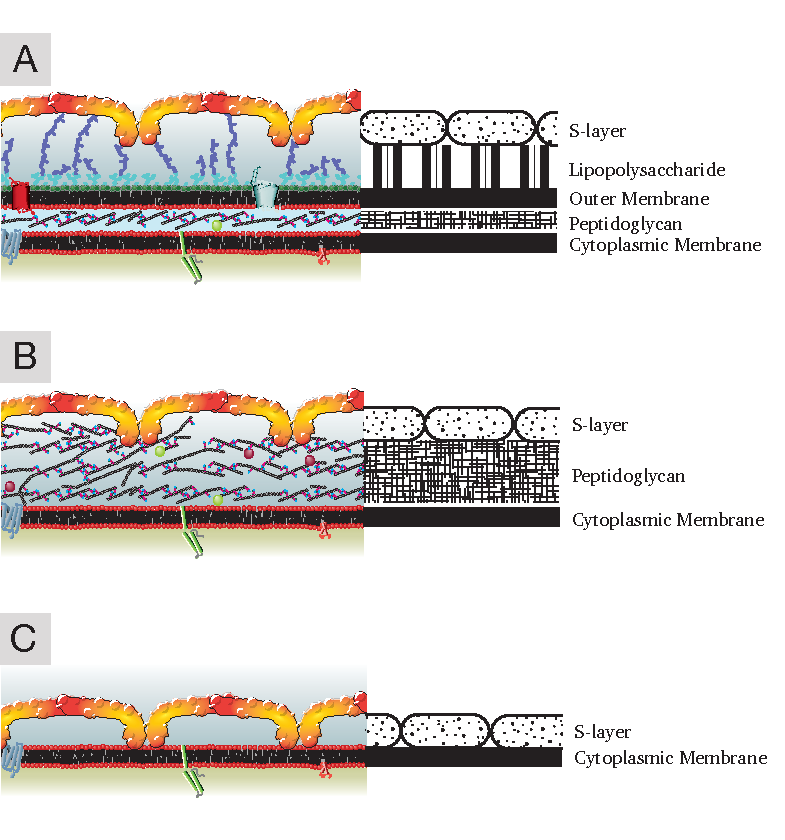
\includegraphics{intro/img/celwalls.pdf}
  \end{center}
  \caption[Cross-sectional diagrams of \ac{S-layer} containing cell envelopes]{Cross-sectional
    diagrams of the cell envelopes of (\textbf{A}) Gram-negative bacteria, (\textbf{B}) Gram
    positive bacteria, and (\textbf{C}) archaebacteria. In all known cases the \ac{S-layer} sits on
    the extreme outer surface of the cell. The left side is a cartoon, artistic interpretation. The right side is a simpler, structural diagram.(This diagram was inspired by Fig. 1 from
    \fullcite{sleytr1983crystalline})}
  \label{fig:cellwalls}
\end{figure}

\Acp{S-layer} are composed of one or only a few proteins or glycoproteins. In most known examples,
\acp{S-layer} are composed of just one repeated protein, in a few cases \acp{S-layer} are composed
of a few separate proteins, which are stacked one on the other. The \ac{S-layer} from \textit{Clostridium difficile} is composed of two
proteins (HMW and LMW) that arise from the cleavage of a single precursor protein (SlpA) that is
cleaved during secretion\upcite[.]{calabi2001difficile, fagan2009difficile} \textit{Bacillus
  anthracis} has a \ac{S-layer} that is composed of two proteins (EA1 and Sap) that are individually
expressed and assemble together on the surface of the bacterium\upcite[.]{mesnage1997molecular}
Interestingly, \textit{Brevibacillus brevis} appears to have two \acp{S-layer} stacked on top of each
other; the outer layer having oblique symmetry and the inner layer having hexagonal
symmetry\upcite[.]{sara1990brevis}
    
For \acp{S-layer} that are composed of a single protein, that protein is repeated thousands of times
across the surface of the cell and is arranged in a regular geometric pattern. The geometric
patterns can be observed by electron microscopy. The traditional electron microscopy techniques of freeze fracture and negative stain have been the most successful techniques historically to see \acp{S-layer} and \ac{S-layer} geometries\upcite[.]{smit1981periodic} In fact, the discovery of \acp{S-layer} and the first image of an \ac{S-layer} published was produced by negative stain electron microscopy\upcite[.]{firstslayer} That first \ac{S-layer} image can be seen in \cref{fig:firstslayer}. For a historical overview of \ac{S-layer} discoveries, refer to Sleytr \etal, 2014\upcite[.]{sleytr2014s}

\begin{figure}[p] % First S-layer
  \begin{center}
    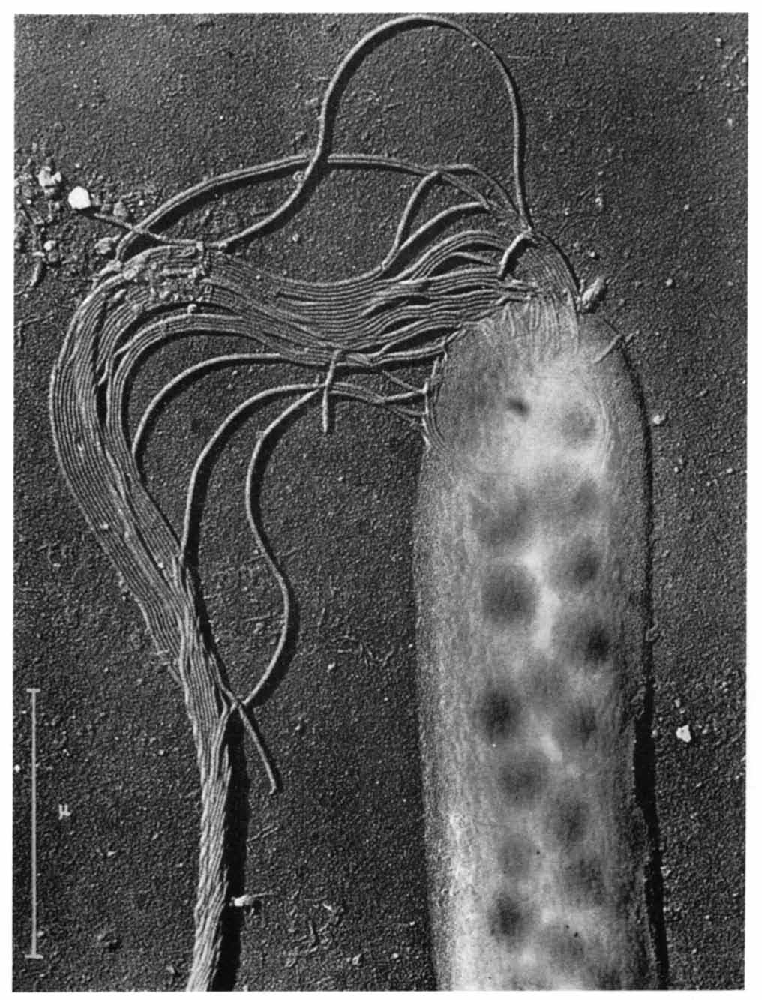
\includegraphics{intro/img/firstslayer.pdf}
  \end{center}
  \caption[The first published image of a \ac{S-layer}]{The first published image of a
    \ac{S-layer}. The hexagonal \ac{S-layer} on the surface of the bacterium --- probably
    \textit{Spirillum} sp. --- is visible along the edges of the cell body (centre right). The scale
    bar denotes one micrometre. (This image is Figure 1 from \fullcite{firstslayer}. Reused with
    full permission from the publisher, Elsevier.)}
  \label{fig:firstslayer}
\end{figure} 

The six major geometric symmetries found in
\acp{S-layer} are oblique (p1 and p2), triangular (p3), rectangular (p4), and hexagonal
(p6). \Cref{fig:symmetries}  features simple examples of the six major
symmetries found in \acp{S-layer}.  Examples of bacteria with oblique \acp{S-layer} are
\textit{Bacillus stearothermophilus} NRS2004$/$3a\upcite{messner1986characterization} and
\textit{Brevibacillus brevis}\upcite[.]{masuda1980reassembly} Examples of bacteria with rectangular
\acp{S-layer} are \textit{Corynebacterium
  diptheriae}e\upcite{kawata1972extracellular} and \acl{aeromonas}
A450\upcite[.]{ishiguro1981loss} An example of a bacterium with a
triangular \ac{S-layer} is \textit{Sulfolobus acidocaldarius}\upcite[.]{weiss1974subunit} Examples
of bacteria with hexagonal \acp{S-layer} are \textit{Bacillus anthracis}\upcite{holt1969comparative}
and \textit{Caulobacter crescentus} CB15\upcite[.]{smit1981periodic}

\begin{figure}[htb] % S-layer symmetries
  \begin{center}
    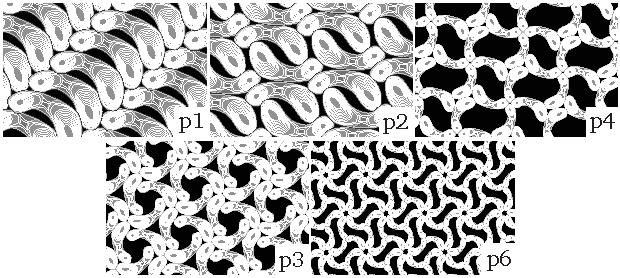
\includegraphics[]{intro/img/symmetries.pdf}
  \end{center}
  \caption[A simple overview of \ac{S-layer} symmetries]{A simple overview of \ac{S-layer}
    symmetries. p1 and p2 are oblique symmetries.  p4 is a rectangular symmetry.  p3 is a triangular
    symmetry.  p6 is a hexagonal symmetry.}
  \label{fig:symmetries}
\end{figure}
   
In addition to the traditional transmission electron microscopy techniques that have been used to
visualize bacterial cell surfaces in the past, a new method of cryo-electron tomography has been
used recently to observe and dissect bacterial cells. Cryo-electron tomography has the advantage
that it can be used to observe unfixed and unstained intact cells. Being a tomographical technique cross
sections can be reconstructed to observe the fine structure within and on a bacterial cell. No
deliberate study has been taken to use cryo-electron tomography to study \acp{S-layer}, but their
presence is easily observed in the fantastic images produced by other studies utilizing the
technique. This technique has been pioneered for use in bacteria and specifically in \ac{caulobacter} by the laboratory of Dr.\,Grant Jensen at the California Institute of Technology. \Cref{fig:intro-tomo}  features a tomographical cross-section of a \ac{caulobacter} cell; visible is the inner and outer membranes and the \ac{S-layer} composed of the protein RsaA.

\begin{figure}[htb]
  \begin{center}
    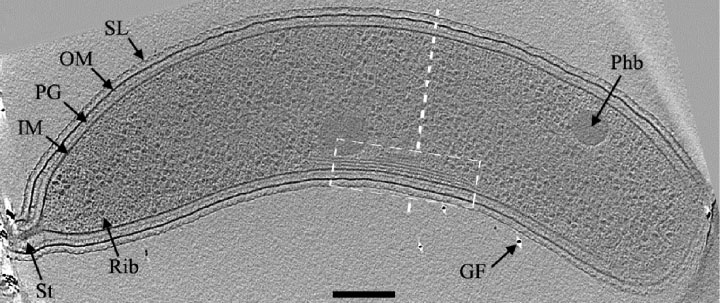
\includegraphics[width=0.8\textwidth]{intro/img/jensentomograph.jpg}
  \end{center}
  \caption[Electrotomograph of \ac{caulobacter}]{ The location of the \ac{S-layer} is around the
    exterior of the cell, as can be seen in this image. The figure is a 19 \si{\nano\meter}
    cross-section through the three-dimensional reconstruction of one representative
    \ac{caulobacter} cell: \textbf{SL}, surface layer;
    \textbf{OM}, outer membrane; \textbf{PG}, peptidoglycan layer; \textbf{IM}, inner membrane;
    \textbf{St}, stalk; \textbf{Rib}, probable ribosome; \textbf{GF}, gold fiducial used to align
    images; \textbf{Phb}, putative poly-$\beta$-hydroxybutyrate granule. The scale bar indicates 200 \si{\nano\meter}.  (This figure is a portion of Figure 1 from \fullcite{Jensen2006tomo}. Reused
    with full permission from the publisher, Wiley. The dotted white lines highlight the location of filaments of the protein Crescentin, the focus of the originating paper. )}
  \label{fig:intro-tomo}
\end{figure}

\subsection{S-layer proteins} \label{sub:intro-slayerproteins} % S-layer protein subsection

Discussing \ac{S-layer} proteins on a whole can be difficult because \ac{S-layer} proteins don't represent a monophyletic group of related molecules; \ac{S-layer} proteins seem to be distinctly unrelated proteins that share a common cellular location and gross structure through convergent evolution. One of the best reviews on \ac{S-layer} proteins was published in 2000 by Margit S\'{a}ra and Uwe B. Sleytr\upcite[.]{sara2000s} 

\ac{S-layer} proteins do tend to share similar properties and overall composition. \ac{S-layer} proteins are relatively large proteins. For the \ac{S-layer} proteins whose sequences are known, all are larger than 400 \acp{aa} and many of them larger than 1000 \acp{aa}\upcite[.]{sara2000s} The amino acids in \ac{S-layer} proteins are rich in hydrophobic and negatively charged residues, low in methionines, and  cysteines are almost completely unrepresented\upcite[.]{gilchrist1992nucleotide, sara2000s, vilen2009surface}  

The most well studied \ac{S-layer} proteins RsaA from \caulobacter{}, SbsB from \ac{geo}, and SbsC also an \ac{S-layer} from \ac{geo}. RsaA is studied for its potential as a biotechnology platform. SbsB and SbsC also have potential for applications but they are well studied because they are easy to work with; they can be expressed in \ecoli{} and will readily form \acp{S-layer} on almost any flat surface available. The ease of working with SbsB has paid off in the form of the first, and only, atomic-level resolution crystal structure of a bacterial \ac{S-layer} protein with the symmetry determining domains intact\upcite[.]{baranova2012sbsb} The protein SbsB was crystallized by inhibiting its \ac{S-layer} forming ability by binding it with a nanobody, a monoclonal single domain camelid antibody. The crystal study reveals that calcium ions play an integral role in the structure of the \ac{S-layer} protein. These calcium ions `trigger' the folding of the protein, this mirrors the hypothesized role of \ac{rtx} motifs in the \caulobacter{} \ac{S-layer} protein RsaA discussed \vpageref{sec:repeat-toxin-motifs}. For our efforts to crystallize RsaA, see \cref{ch:crystal} \vpageref{ch:crystal}.
 
\ac{S-layer} proteins are almost universally glycosylated in \textit{Archaeabacteria}, commonly
glycosylated in Gram-positive bacteria, and very rarely glycosylated in Gram-negative
bacteria\upcite[.]{sara2000s, lechner1989structure}
For some microbes, the \ac{S-layer}'s main function may be as a platform for oligo/polysaccharide chains. One study by Sch\"{a}ffer et\,al.~asked the question about the glycosylation of \ac{S-layer} proteins, ``Are \ac{S-layer} Glycoproteins and Lipopolysaccharide Related?''\upcite[]{schaffer1996s} The study identified structural similarities between the carbohydrates in \ac{OPS} and the carbohydrates on glycosylated \ac{S-layer} proteins; pointing out they have more in common with each other than with eukaryotic polysaccharides. The study makes flawed leaps from sugar structures to phylogenetic and taxonomic conclusions, but the study does highlight that supporting a highly glycosylated surface is a widespread feature in microbial life and it is a role that \ac{S-layer} proteins serve in some organisms. 
% subsection s_layer_structure (end) 

  \subsection{Functions of S-layers}
  \label{sec:intro-slayersfunction}

  As mentioned before, \acp{S-layer} are not a single family of related proteins---likewise they do not fill the same needs in all species. Interestingly, despite the apparent convergent evolution in many disparate organisms pushing towards a widespread similarity in structure and composition, \acp{S-layer} seemingly perform many  different functions. Further, \acp{S-layer} require a large metabolic commitment to produce and maintain, despite that, they are still retained in many species where their functions are enigmatic. Due to their location on the cell surface, \acp{S-layer} are undoubtly invloved wtih the a cell's interaction with the environment. While the classification of \ac{S-layer}-possessing bacteria into pathogenic versus non-pathogenic can be somewhat arbitrary, it is a convenient distinction to make and use to compare \ac{S-layer} functions. 
  
  \paragraph{Pathogenic bacteria} For pathogenic bacteria, a \ac{S-layer} is often a virulence factor. In \ac{anthrax}, the \ac{S-layer} consists of the protein BslA and it functions as an adhesin\upcite[.]{kern2010bsla} BslA is sufficient and required for \ac{anthrax} to adhere to host cells and mutants that lack the \ac{S-layer} have much reduced virulence and increased time-to-death in animal models. Due to their location on the surface of the cell, \acp{S-layer} functioning as adhesins is a common theme in pathogens. \ac{aeromonas} has a \ac{S-layer} that also functions as an adhesin\upcite[.]{garduno2000host} The \ac{aeromonas} \ac{S-layer} binds to both fibronectin and laminin on host cell surfaces\upcite[]{doig1992binding} but is not involved or required for host cell invasion, which probably mediated by the \ac{LPS}\upcite[.]{garduno2000host}
  The \ac{aeromonas} \ac{S-layer}, composed of the protein VapA, is sufficient to confer host cell adhesion to the bacterial cells and also to nylon microbeads \textit{in vitro}. 

  For \ac{cfetus}, its \ac{S-layer} is central to its success as a pathogen of ungulates. The \ac{S-layer} of \ac{cfetus} is involved in disseminating the bacteria throughout the host's body and evading the host immune system\upcite[.]{thompson2002campylobacter} The manner in which \ac{cfetus} uses its \ac{S-layer} to escape the immune system is remarkable. The \ac{S-layer} provides the cells with an innate resistance to complement; strains with an intact \ac{S-layer} bound less C3 protein than cells lacking a \ac{S-layer}. By binding less C3, \ac{S-layer} positive \ac{cfetus} prevent complement-mediated killing and opsonization by C3b. The \ac{S-layer} would be a natural target for antibody-mediated adaptive immunity, but \ac{cfetus} has also evolved a strategy to escape antibody recognition. \ac{cfetus} possess the ability to undergo antigenic conversion by expressing different versions of its \ac{S-layer}. The \ac{cfetus} cells can invert portions of their genomic DNA to express alternate \ac{S-layer} proteins and cognate \ac{OPS} anchor molecules. As an example, the \ac{cfetus} serotype A strain 23D encodes for eight different \ac{S-layer} proteins and can switch between expressing each by moving a single active promoter in front of the \ac{S-layer} protein gene to be expressed. These \acp{S-layer} are not just different antigenically, they can even form different symmetry patterns (see \cref{fig:symmetries}).

\paragraph{Non-pathogenic bacteria} \label{sec:non-path-bact} %% Intro paragraph
The roles of \acp{S-layer} in non-pathogenic bacteria can often be mysterious in lab settings. While virulence can be a clear, quantifiable phenotype, the fitness gain derived from an \ac{S-layer} in the wild is not often abundantly obvious in a test tube. \acp{S-layer} have been shown to act as barriers to the outside world.
\acp{S-layer} acting as a physical barrier, protecting the cell, is a function primarily exemplified by \caulobacter and other Gram-negative bacteria possessing an \ac{S-layer}. Susan Koval of the University of Western Ontario has done extensive research into the biology and life-cycle of \textit{Bdellovibrio} spp. and \textit{Bdellovibrio}-like species, predatory bacteria that prey on gram-negative bacteria like \caulobacter. Koval showed that the \ac{S-layer} of \caulobacter had a protective effect against \textit{Bdellovibrio} predation\upcite[.]{koval1991effect} This protective effect was seen for  \ac{aeromonas}, \textit{Aquaspirillum serpens}, \textit{Aquaspirillum sinuosum}, \ac{cfetus}, and \caulobacter. On the other hand, \acp{S-layer} do not confer any protection from predation by protozoans (\eg{} \textit{Tetrahymena thermophila} and \textit{Paraphysomonas vestita})\upcite[.]{koval1993predation} The barrier capacity of \acp{S-layer} extends to blocking abiotic threats, as was demonstrated by De la Fuente-N{\'u}{\~n}ez \etal in \caulobacter 2012. \caulobacter cells that possessed an \ac{S-layer} were found to have protection against the effects of antimicrobial peptides compared to cells that lack an \ac{S-layer}\upcite[.]{de2012bacterial} The authors note that the peptides were smaller than the pores in \caulobacter \ac{S-layer} (see \cref{fig:intro-micrograph}) and yet the protective effect existed. The \ac{S-layer} may act as a sponge, not just a physical barrier, adsorbing harmful molecules before they can reach the cell. The \ac{S-layer} of \caulobacter{} is not glycosylated but many other species' \acp{S-layer} are glycosylated and those carbohydrates would add another layer of coating to the cell to ward off intrusion.

% Due to their location around the outside of a cell, \acp{S-layer} are in a prime position to modify the surface the chemical and physical characteristics of a microbe.

A protein coating is going to impart a cell surface with different properties than a `naked' cell, these differences may be a conserved function of an \ac{S-layer}.
 It has been noted that many bacteria with an \ac{S-layer} are more hydrophobic than isogenic variants lacking an \ac{S-layer}\upcite[.]{beveridge1997v} A noted exception to the hydrophobicity observations was for \caulobacter strains CB2A and CB2NY66R, possibly its \ac{S-layer} covers beneath it a more hydrophobic outer membrane (see \cref{ch:lps} on \cpageref{ch:lps} for our research on the \caulobacter \ac{LPS}). Beyond changing the general chemical properties of the cell surface, \acp{S-layer} also change the cell surface to provide a specific site for extracellular proteins to anchor. Enzymes that are secreted, but remain associated with the cell, can use \acp{S-layer} as display platforms. The enzyme pullulanase in \textit{Clostridium thermosulfurogenes} anchors itself into the \ac{S-layer} with three C-terminal regions that have a significant sequence homology to the \textit{C. thermosulfurogenes} \ac{S-layer} protein\upcite[.]{matuschek1994pullulanase} It is thought that the \textit{C. thermosulfurogenes} pullulanase integrates itself in the lattice of the \ac{S-layer} in order to anchor itself. Intergration into the \ac{S-layer} is not the strategy used by \ac{geo} DSM2358 and its amylases. The high molecular weight amylase from \textit{G. stearothermophilus} binds the cell surface but without any detectable interaction with peptidoglycan, instead it associates with \ac{S-layer} in a manner that is specifically not lattice integration\upcite[.]{egelseer1995s}

% \subsection{History of S-layers} % (fold)
% \label{sub:history_of_s_layers} % Do I need a history section??

\subsection{RsaA} \label{sec:intro-rsaa}

RsaA, named for \underline{r}egular \underline{s}urface \underline{a}rray\upcite[,]{gilchrist1991transformation} is a 1026 \ac{aa} protein from \caulobacter with an average \ac{mw} of 98001.70 Da and an \ac{pi} of 3.85. The amino acid sequence of RsaA can be found in the appendix on \cpageref{app:rsaseq}. The \ac{S-layer} of \caulobacter comprises roughly 45000 copies\upcite[]{slayercryo} of RsaA arranged in an p6 symmetry (see \cref{fig:symmetries}). RsaA is a \ac{t1ss} secreted protein containing five to six \ac{rtx} motifs.

\Cref{fig:intro-micrograph} displays a computer reconstructed view of the surface of the \ac{S-layer} of \caulobacter as determined by tilt-tomography electron microscopy\upcite[,]{smit1992s} this figure is the highest resolution image we have for the structure of RsaA and the \ac{S-layer}, a resolution of about 20 \AA{}. 
In a very elegant series of experiments in 2010, Amat \etal were able to determine the configuration of the RsaA monomers in \ac{S-layer} structure\upcite[.]{slayercryo} Different constructs of RsaA were produced that contained single cysteine residues at different locations throughout the protein.  Labelling those cysteines with nano-gold particles, \textit{in situ} in the \ac{S-layer}, led to noticeable differences in electron density in hexagonal unit cell of the \ac{S-layer}. These densities corresponded to the physical locations of the engineered cysteine residues. This work proved that the N-termini of the RsaA monomers are  located in the axis of three-fold symmetry, while the C-termini are centered around the axis of the six-fold symmetry (refer to \cref{fig:intro-micrograph})

\begin{figure}[htb]
  \begin{center}
    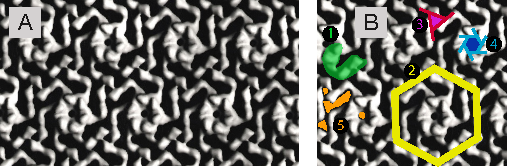
\includegraphics[width=\textwidth]{intro/img/slayermicrograph.pdf}
  \end{center}
  \caption[Reconstructed surface of the \caulobacter \ac{S-layer}]{
    The surface structure of the \ac{S-layer} from \caulobacter, reconstructed from tilt-series electron microscopy. \textbf{A.} A section of reconstructed surface of the \caulobacter \ac{S-layer}. The image shown is in a left-handed configuration, except the handedness of the \ac{S-layer} couldn't be determined in the original study, therefore this image may be a mirror image of the true configuration of the \ac{S-layer}. \textbf{B.} Interpretations of the micrograph.  A monomer of RsaA is highlighted in green (\textit{B.1}).  The unit cell of the \ac{S-layer} is six copies of RsaA arranged in a hexagonal pattern (\textit{B.2}).  The center of three-fold symmetry, red, is comprised of the N-termini of RsaA (\textit{B.3}).  The C-termini of the RsaA monomers face towards each other in the center of the point of six-fold symmetry, blue (\textit{B.4}). Possible pores through the \ac{S-layer} are highlighted in orange (\textit{B.5}). (This image is derived from Figure 6 from \fullcite{smit1992s})
  }
  \label{fig:intro-micrograph}
\end{figure}   

\paragraph{Type 1 secretion} RsaA is secreted by a \ac{t1ss}. \Ac{t1ss} secreted proteins are secreted in one step across both the inner and outer membranes of Gram-negative bacteria\upcite[.]{holland2005type} A \ac{t1ss} requires three components: an inner membrane spanning \ac{abc} transporter, a periplasm spanning membrane fusion protein, and an outer membrane protein. For RsaA's secretion from \caulobacter, these proteins are RsaD, RsaE, and RsaF (either RsaFa or RsaFb)\upcite[.]{awramabctransport, rsaf} Like all \ac{t1ss} secreted proteins, RsaA is secreted starting from the C-terminus to the N-terminus. As proteins are translated from the N-terminus to the C-terminus, all \ac{t1ss} secreted proteins (including RsaA) exist in the cytoplasm as fully translated polypeptides prior to secretion. This is in contrast to protein secreted by N-terminus first means, which allow for the possibility for secretion to begin on a nascent peptide before translation is complete. The diameter of \ac{t1ss} pore is not wide enough to accommodate the secretion of a fully folded protein, so \ac{t1ss} secreted proteins often have a C-terminus that is intrinsically disordered prior to secretion; this disordered state is mediated by \ac{rtx} motifs\upcite[.]{chenal2009rtx}   

  \paragraph{Repeat-in-toxin motifs} \label{sec:repeat-toxin-motifs} First identified in the \ecoli protein $\alpha$-haemolysin (HlyA)\upcite[,]{felmlee1988alterations} \ac{rtx} motifs are a nearly ubiquitous component of \ac{t1ss} secreted proteins. Despite the name, \acl{rtx} aren't exclusively found in toxins, they are found in many classes of protein, lipases, proteases, S-layers,\textit{etc.}  \ac{rtx} motifs are small peptide sequences, typically 6--9 \ac{aa} in length, the amino acid sequence is \texttt{GGXGXD}\upcite[]{letoffe1992secretion} or \texttt{GGXGXDXLX}(where \texttt{G} is glycine, \texttt{D} is aspartate, \texttt{X} can be any amino acid, and \texttt{L} is leucine but is often substituted for valine, isoleucine, phenylalanine, or tyrosine)\upcite[.]{rose1995interaction, chenal2009rtx} The short sequences are always present in multiples (6--50+), often found in tandem repeats. Each \ac{rtx} motif forms two half sites for binding \ce{Ca^2+}, which can collaborate with other neighbouring \ac{rtx} sites to coordinate ions and stabilize a connection between disparate regions of a protein. Upon binding \ce{Ca^2+}, \ac{rtx} motifs assume a parallel $\beta$-roll fold\upcite[,]{meier2007calcium} rolling around \ce{Ca^2+} ions at the turns. An example of a \ac{rtx} $\beta$-roll structure can be found in \cref{fig:intro-rtx}.

  \begin{figure}[htb]
    \begin{center}
      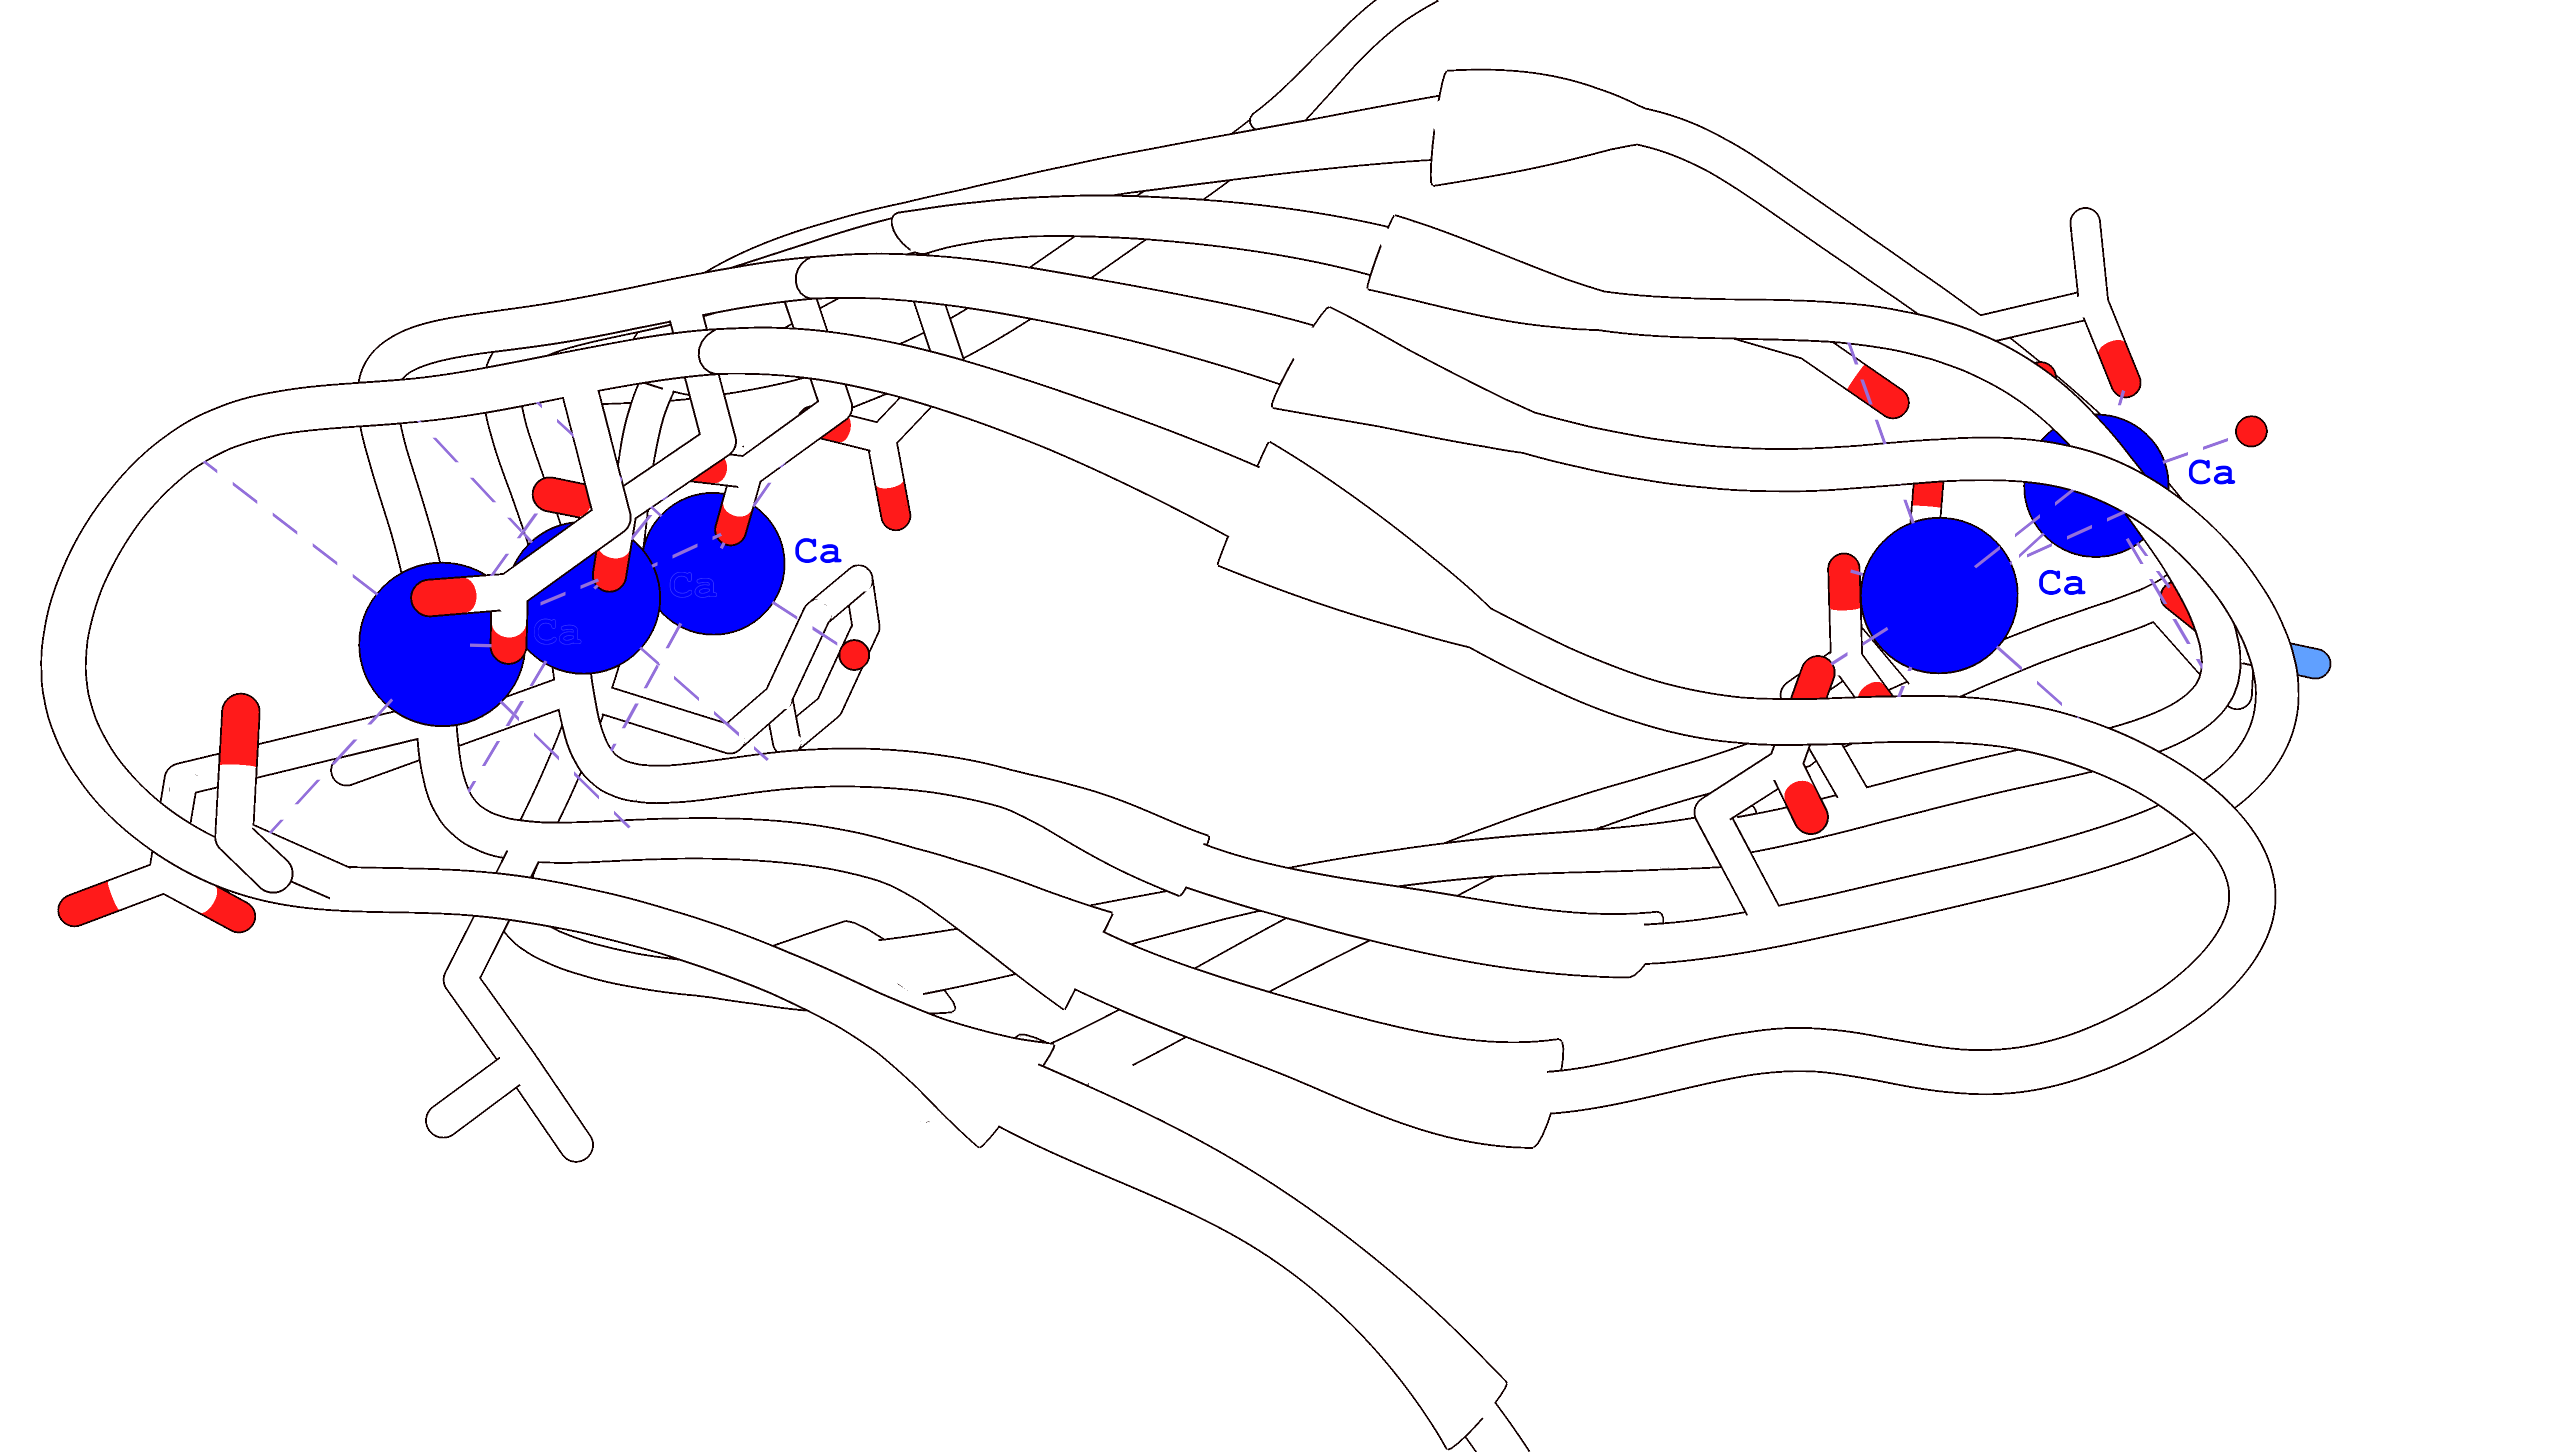
\includegraphics[width=0.7\textwidth]{intro/img/rtx-white.png}
    \end{center}
    \caption[The structure of \ac{rtx} motifs]{The structure of \ac{rtx} motifs. This view is down the barrel of an \ac{rtx} $\beta$-fold. The blue spheres are calcium ions coordinated by aspartate residues which are shown. This structure is of MIS38, an extracellular lipase from \ac{pseudomonas} (PDB:2Z8X). The structure here depicts five \ac{rtx} sites binding five \ce{Ca^2+} ions, RsaA from \caulobacter also has five \ac{rtx} motifs in close vicinity and my have a similar structure the presented structure above. See the sequence of RsaA on \cpageref{app:rsaseq}, \ac{rtx} sequences are bolded. Generated using the program \texttt{Chimera} (\fullcite{pettersen2004ucsf}).
    }
    \label{fig:intro-rtx}
  \end{figure}   

  \ac{rtx} motifs are always on the C-terminal side of \ac{t1ss} proteins, and are thus are in the leading part of the polypeptide to be loaded into the secretion machinery and the first part to be secreted. It should be noted that bacterial intracellular \ce{Ca^2+} concentrations are extremely low, 90$\pm$10 \si{\nano\molar}, and extracellular \ce{Ca^2+} concentrations are higher, 0.1--1 \millimolar\upcite[.]{gangola1987maintenance, norris1996calcium} It is thought that the roles of \ac{rtx} motifs in \ac{t1ss} proteins are to induce an intrinsically disordered C-terminus prior to secretion and to quickly  bind \ce{Ca^2+} and begin folding once the protein has started to emerge from the secretion machinery\upcite[.]{perez2010characterization, sotomayor2014disorder} The calcium-induced folding may help the thermodynamics of secretion, possibly assisting by pulling the protein out of the pore.  Despite the apparent importance of \ac{rtx} motifs in \ac{t1ss} proteins, they are not sufficient nor even necessary for secretion\upcite[]{felmlee1988alterations} but in at least the case of HlyA, in \ecoli, the \ac{rtx} repeats are required for proper folding, activity, and maximal secretion\upcite[.]{felmlee1988alterations} It has been thought that the folding of the \ac{rtx} motifs can act as an `intramolecular' chaperone; they fold quickly first then act as a nucleation point for the rest of the protein to fold on\upcite[.]{sotomayor2014disorder} 
 
  \subsection{Biotechnology applications of S-layers}\label{sec:biot-appl-s} 
  
  \Acp{S-layer}' ability to self-assemble into large, complex structures makes them  an attractive platform for biotechnological applications. Their density and regular arrangement over relatively large distances is unique in biology. There have been many groups pursuing technologies that utilize \acp{S-layer} assembled off of the surface of the cell and groups that focus on \ac{S-layer} technologies on the cell surface. Many different technologies have been developed.
  One of the significant defining difference between all \ac{S-layer} applications is the location the \ac{S-layer} is assembled. The potential sites for assembly are:
  \begin{itemize}
  \item In suspension
  \item On a solid surface
  \item On a liquid interface of lipid membrane
  \item On a lipid nanoparticle
  \item On a cell surface
  \end{itemize}
  % In their 1997 review of  \ac{S-layer} applications, authors Uwe Sleytr and Margit S{\'a}ra categorize the potential applications for \acp{S-layer}\upcite[]{sleytr1997bacterial}:
  % \begin{itemize}
  % \item \ac{S-layer} ultrafiltration membranes
  % \item \ac{S-layer} supported lipid membranes and films
  % \item \ac{S-layer} mircoparticles
  % \item \acp{S-layer} as matrices for biomineralization and particulate organization %Kinda a shitty word
  % \item Genetically modified \acp{S-layer} for displaying peptides
  % \end{itemize}

  Very little interest or work has been done on developing applications for \acp{S-layer} that assemble and exist in liquid suspension. \Acp{S-layer} are inherently two-dimensional and unrestricted freedom in liquid suspension does not highlight their unique structure. Assembling \acp{S-layer} in solution is most often a means to getting the \acp{S-layer} onto a solid surface. Once on an assemble \ac{S-layer} is on a solid surface it is a potent structure for biotech development. The \ac{S-layer} itself can act as a filter or the \ac{S-layer} can be a platform for functionalized molecules and peptides.

  Using \acp{S-layer} as ultrafilters has been a tempting idea since not long after they were discovered. As mentioned \vpageref{sec:non-path-bact}, one of the possible natural functions of \acp{S-layer} is to act as a physical barrier against large, intrusive foreign entities. Unlike conventional ultrafilters made of inorganic polymers, \acp{S-layer} are isoporous with very stringent molecular weight cutoffs. In its most basic inception, an \ac{S-layer} ultrafilter could be constructed by assembling an \ac{S-layer} on the inner surface of a traditional ultrafiltration membrane. These \ac{S-layer} ultrafiltration membranes (sometimes called \textsc{sum}s) do have exquisite selectivity of filtering and when they are crosslinked with glutaraldehyde, they are highly resistant to solvents, acids, and bases\upcite[.]{sara1987production} These \ac{S-layer} filters were covered by at least three US patents, , 4886604, 5028335, but the last of which expired in the year 2011. The apparent lack of enthusiasm in the field of ultrafiltration using \acp{S-layer} in the last few years suggests that the early results weren't easily translatable into a large product.
  
  Having the \ac{S-layer} be a platform for functional molecules and peptides is the most popular approach to using \acp{S-layer}. The most uncomplicated way to introduce a functional structure into an \ac{S-layer} is to genetically clone it into the \ac{S-layer} gene itself. Molecules of interest can always be chemically linked to an intact \ac{S-layer}\upcite[,]{weinert2015synthesis} but the opportunity for \ac{S-layer} to inherently display peptides of interest dominates the field. The best few examples of molecules of interest being attached to an \ac{S-layer} after it is assembled are cases were coupling domains were first cloned into the \ac{S-layer} protein. One such example is streptavidin cloned into SbsB (an \ac{S-layer} protein from \ac{geo}) so that biotinylated molecules could be loaded on to it\upcite[.]{moll2002s} Another example is from the \ac{S-layer} of \caulobacter{}, where protein G has been expressed so that thousands of copies of any IgG antibody can be loaded across its surface\upcite[.]{nomellini2007s}

  As mention just above, genetically modifying \ac{S-layer} genes so that the proteins contain valuable peptides and proteins is the showpiece technology for \acp{S-layer}. These exogenous peptides can be displayed at an incredibly high density across a relatively huge distance by being displayed in an \ac{S-layer}. This approach has been successfully pursued in \caulobacter{}' \ac{S-layer}. The \caulobacter{} \ac{S-layer} has displayed vaccines\upcite[,]{bingle1997expression} enzymes\upcite[,]{bingle1993all} HIV-binding proteins\upcite[,]{nomellini2010development, hivmicrobicide2} and peptides for biosorption of heavy metals\upcite[.]{patel2010genetic} 

  All \acp{S-layer} are biological entities that are ultimately tethered to a cell membrane, but if that arrangement is flipped a lipid membrane can be formed and supported by an \ac{S-layer}\upcite[.]{pum1993large} Two-dimensional lipid-membrane structures can also be turned into three-dimensional \ac{S-layer}-coated nanoparticles\upcite[.]{kupcu1995liposomes} The two-dimensional structures can be assembled across the surface of a Langmuir-Blodgett apparatus. The majority of the interest in these structures is in the lipid layer\upcite[,]{schuster2000s} the \ac{S-layer} only acts as a stabilizer. On the other hand, lipid nanoparticles coated in \acp{S-layer} garner a great deal of excitement for for the \ac{S-layer} itself. The promise of lipid nanoparticles (\ie{} vesicles, liposomes and solid-cored particles) is that all the above technology already developed or being currently developed can be translated to an abiotic particle that highlights the strengths of \acp{S-layer}. Some \acp{S-layer} will readily assemble on nearly any surface, those \acp{S-layer} will coat standard lipid vesicles that are present\upcite[,]{ucisik2015s} while other \acp{S-layer} require specialized lipids to assemble upon a nanoparticle. For instance, \caulobacter \ac{S-layer} can be reassembled on to lipid vesicles composed of \caulobacter{} \ac{LPS}\upcite[.]{nomellini1997factors} 
  
  Two good reviews on the subject of \ac{S-layer} applications are written by Smit (2008)\upcite[]{smit2008heads} and Ilk, Egelseer, and Sleytr (2011)\upcite[.]{ilk2011s}
  % The long-range uniformity of \acp{S-layer} whet the interest for the structures that can be built on top of them. In this vein, using \acp{S-layer} to support mineralization, nanoparticle arrangement, and lipid membranes all share in common using \acp{S-layer} as physical structures.
% Many \acp{S-layer} can assemble themselves into long-range regular structures \textit{in vitro}, unattached to a cell surface. These ``\textit{in vitro} \acp{S-layer}'' are a hotbed for biotechnology development because they provide a uniquely dense and patterned protein surface that can be divorced from contaminants of whole cells. 
% Undoubtedly, the driving force behind these \acp{S-layer} has been Dr.\,Uwe~B.~Sleytr, professor of nanobiotechnology at the University of Natural~Resources and Life~Sciences at Vienna, Austria. Dr. Sleytr's work has focused on the  

\section{Lipopolysaccharide}\label{sec:intro-lps}
% Intro and overview of LPS
% 1. Structure
% 2. Location
% 3. Role
The most abundant non-protein  component of the Gram negative outer membrane is
\ac{LPS}. The \acp{LPS} of \ecoli and \ac{salmonella} are regarded as the
``canonical'' examples. Those \acp{LPS} are the molecules that all others are
compared against and this thesis will do the same. 

\Ac{LPS} resides in the outer leaflet of the Gram negative outer membrane. In
physiological conditions, in wild-type bacteria \ac{LPS} is the only lipid
component in the outer leaflet\upcite[.]{smit1975outer, kamio1976outer}. 

\Ac{LPS} is synthesized in the inner membrane. While in wild type cells there
exists detectable levels of \ac{LPS} in the inner membrane, the vast majority of
\ac{LPS} resides in the outer membrane\upcite[.]{polissi1996mutational, ding1976separation} Fully
formed \ac{LPS} is transported across the periplasm to the outer membrane via
the proteins LptABCDE\upcite[.]{sperandeo2007characterization,
  ruiz2008identification} The exact details of how a large \ac{LPS} molecule can
traverse the periplasm and be inserted into the outer leaflet are still cloudy;
the difficulty is in no small part due to the fact that all the required proteins
are essential for life.

\Cref{fig:lpsoverview} highlights a simplified \ac{LPS} structure from
\textit{Salmonella minnesota} as reported by Vukajlovich, Hoffman, and Morrison (1987)\upcite[.]{vukajlovich1987activation}  There are three fundamental components of \ac{LPS}: lipid A, the core oligosaccharide, and the O-polysaccharide. 
\begin{figure}[p]
  	\begin{center}
   		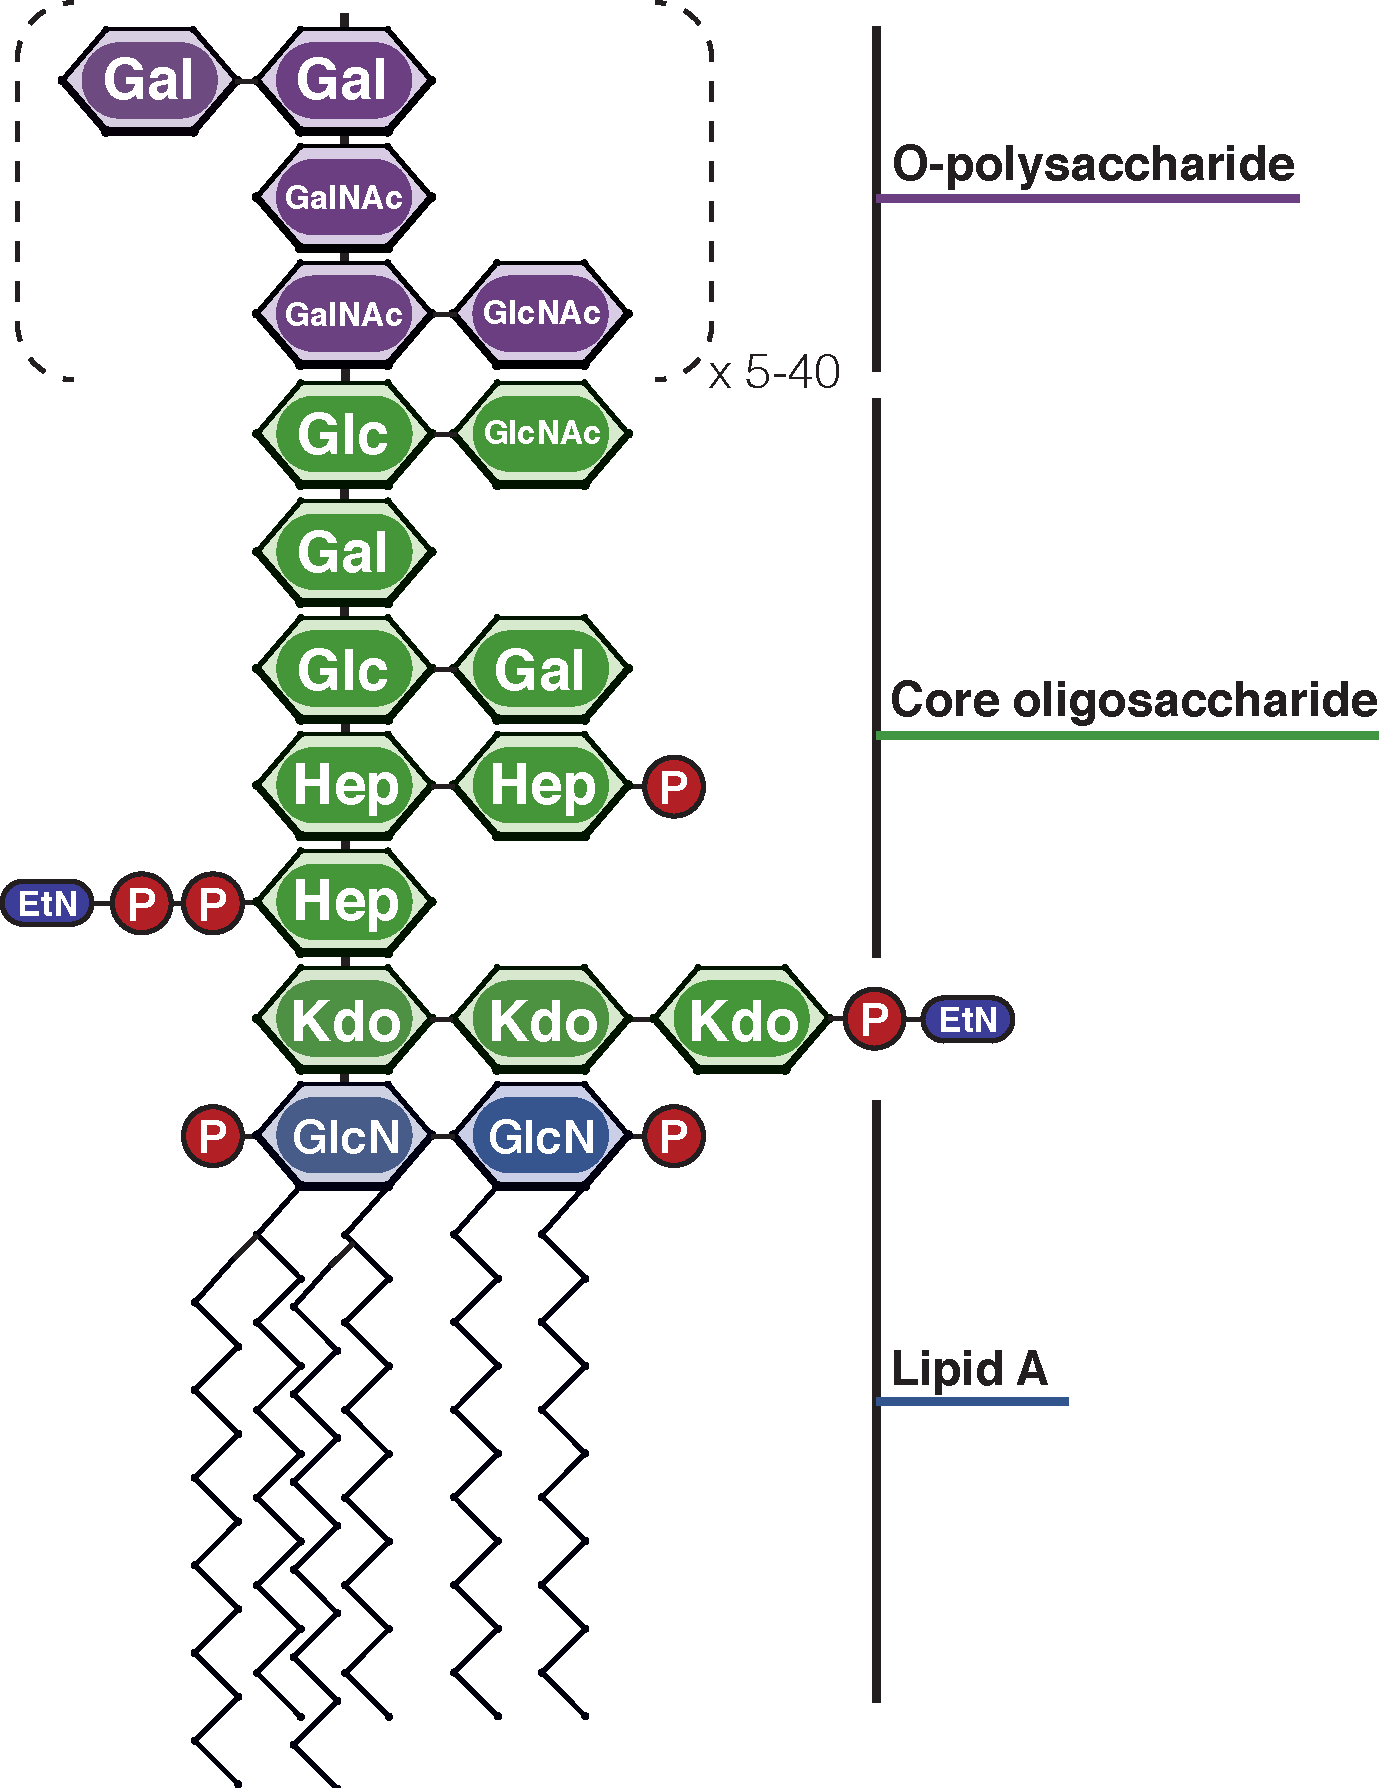
\includegraphics[width=0.7\textwidth]{intro/img/lpsoverview.pdf}
   	\end{center}
   	\caption[Simplified structure of \ac{LPS} from \ecoli~O111:B4]{
The wild type \ac{LPS} from \textit{Salmonella minnesota}. The lipid A is at the
bottom of the figure (in blue), it comprises a backbone of two glucosamine residues. Each
glucosamine has an attached phosphate moeity and  three fully saturated acyl
chains. Above the lipid A is the core oligosaccharide (in green). This core
oligosaccharide is a hendecasaccharide. Extending from the core oligosaccharide
is the \ac{OPS} (in purple). The structure of this \ac{OPS} is a variable number of
pentasaccharide subunits (5--40). Abbreviations: Glc, glucose; GlcN, glucosamine; GlcNAc,
N-acetylglucosamine; Gal, galactose;  GalNAc, N-acetylgalactosamine; Kdo,
3-deoxy-\textsc{d}-\textit{manno}octulosonic acid; Hep,
\textsc{l}-\textit{glycero}-\textsc{d}-\textit{manno}heptose; P, phosphate; and
EtN, ethanolamine.
}
   	\label{fig:lpsoverview}
\end{figure}   

  \subsection{Lipid A}\label{sec:lipidA-intro}
  
    \paragraph{Structure}
    
    Lipid A is the `base' of the \ac{LPS} molecule. The backbone of canonical \acp{LPS} is two glucosamine sugars bound to each other by an $\beta$1$\rightarrow$6 bond. The diglucosamine molecule has two O-linked beta hydroxy acyl chains at the C-3 and C-3$^\prime$ positions and two N-linked beta hydroxy acyl chains at the C-2 and C-2$^\prime$ positions. The two `prime' acyl chains are modified with subsequent acyl chains attached at the beta hydroxy groups. All these acyl chains are fully saturated.
    
    The C-1 and C-4$^\prime$ positions of the diglucosamine are phosphorylated. These phosphates give the lipid A a net negative charge and they are thought to bind divalent cations which form electrostatic bridges with neighbouring lipid A molecules and stabilize the outer membrane\upcite[.]{leive65, leive1974barrier}

    The C-6$^\prime$ postion is ligated to the core oligosaccharide. The canonical structure has the C-6$^\prime$ position occupied with an $\alpha$2$\rightarrow$6 bond to a Kdo sugar.

    \Cref{fig:lipidA} shows this canonical structure as it is found in \ecoli K12.

\begin{figure}[htb]
  	\begin{center}
   		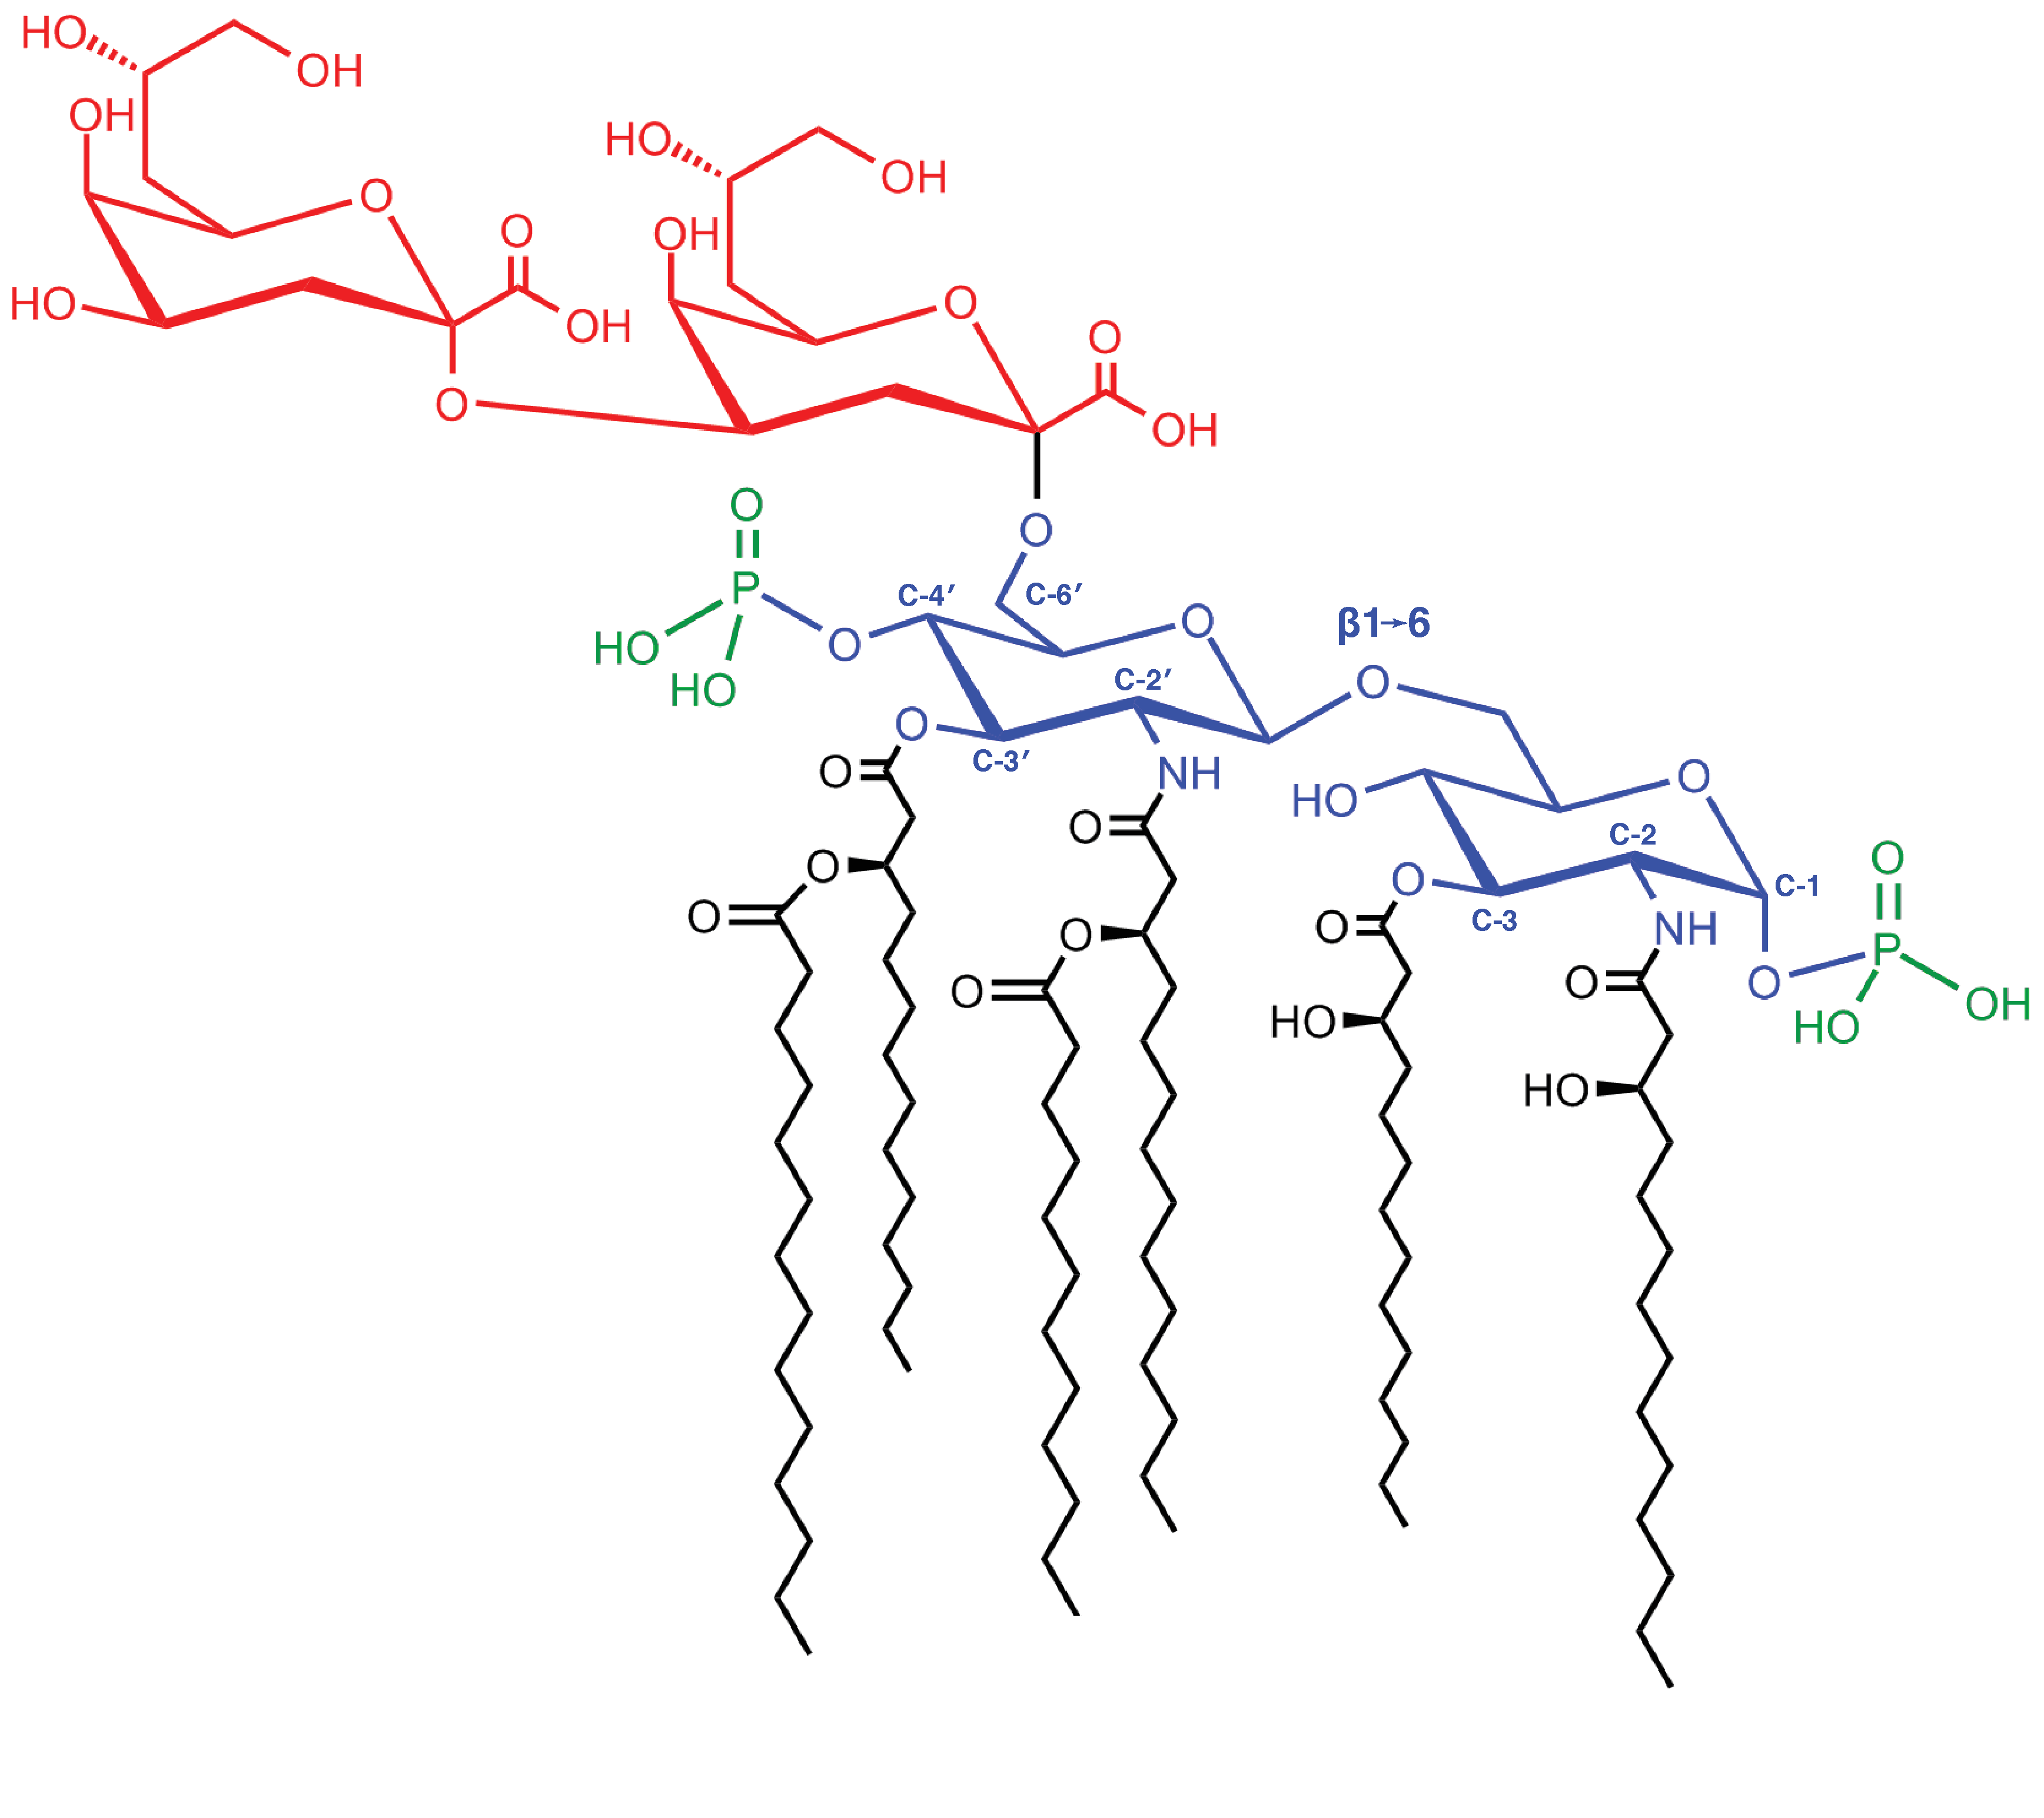
\includegraphics[width=0.6\textwidth]{intro/img/lipidA.pdf}
   	\end{center}
\label{fig:lipidA}
   	\caption[Kdo$_{2}$-Lipid A from \ecoli K12]{ 
Kdo$_{2}$-Lipid A from \ecoli K12. The lipid A portion comprises the phosphates (green), the glucosamines (blue), and the acyl chains (black). The two Kdo sugars present are the start of core oligosaccharide.
}
\end{figure}   

Many, Lipid A structures that differ from the canonical structure. Examples exist of modified structures at all the possible locations: the phosphates, the glucosamines, and the lipids. An excellent review on lipid A modifications is by Raetz et al.~(2007)\upcite[.]{raetz2007lipid}

 The phosphate modifications are often extra chemical groups linked directly to the phosphates. Anionic attachments are common, such as ethanolamine (\eg \textit{Salmonella minnesota}, see \cref{fig:lpsoverview}) and glucosamine (\eg \textit{Bordatella pertusis}\upcite[]{marr2008glucosamine}). Neutral attachments to the phosphate are also possible such as methyl groups (\eg \textit{Leptospira interrogans}\upcite[]{hinckley2005leptospira}). The phosphates can also be removed, examples of lipid A molecules missing a phosphate are \textit{Rhizobium etli}\upcite[,]{que2000two} \textit{Helicobacter pylori}\upcite[,]{tran2004periplasmic} and \textit{Francisella tularensis}\upcite[.]{wang2006structure} Removed phosphates can also be replaced with ethanolamine (\eg \textit{H. pylori}\upcite[]{tran2004periplasmic}) or anionic sugars such as galactosamine (\eg \caulobacter{}\upcite[]{caulobacterlipida} and \textit{R. etli}\upcite[]{que2000two}).
 
Lipid modifications come in the form of the number of acyl chains, the length of the acyl chains, and the inner structure of the acyl chains. Six acyl chains is the standard found in canonical lipid A molecules in enteric bacteria, but the number of fatty acid groups can be as high as eight (\eg \textit{Vibrio cholera} O139\upcite[]{chatterjee2003lipopolysaccharides}) and as low as four (\eg \textit{H. pylori}\upcite[]{tran2004periplasmic}). The lengths of the acyl chains in lipid A do not vary as much as in other lipids due to more stringent acyltransferases, but they do vary between bacteria\upcite[.]{wyckoff1998hydrocarbon} An extreme example is a 28 carbon long acyl chain in \textit{Rhizobium leguminosarum}\upcite[.]{basu2002expression} The acyl chains in lipid A are usually fully saturated but unsaturated examples are not uncommon. Bacteria with unsaturations in their lipid A include \caulobacter{}\upcite[,]{caulobacterlipida} \textit{Yersinia pestis}\upcite[,]{rebeil2004variation} and \textit{Rhodobacter capsulatus}\upcite[.]{krauss1989structural}

    \paragraph{Immunology}

    

  \subsection{Core oligosaccharide}\label{sec:core-oligosaccharide-intro}
  
    \paragraph{Structure}

    \paragraph{Synthesis}

  \subsection{O-polysaccharide}\label{sec:o-polysaccharide}

    \paragraph{Structure}

    \paragraph{Synthesis}
  %%-----------------------------------------------------------------------------%%
  \section{Porins} \label{sec:intro-porins}   
 
The outer membrane of Gram negative bacteria is a particularly impermeable membrane to lipophilic and hydrophylic molecules. In 1976 a protein complex was first isolated from the outer membrane of \ac{salmonella} that produced transmembrane channels which non-specifically transported solutes; this complex was the first to be called a `porin'\upcite[.]{nakae1976outer} Today, the term porin refers to outer membrane proteins that transport molecules across a membrane passively. This definition is for non-specific protein channels\upcite[]{nikaido2003molecular}, like OmpF from \ecoli{}, but sometimes the definition is opened up to structure-specific transport channels, such as LamB in \ecoli\upcite[.]{benz1988structure, hancock1987role} 

Porins act as sieves in the outer membrane allowing small solutes to pass from the environment to the periplasm. Without a channel for them to pass, the outer membrane would be impermeable to these usually hydrophilic nutrient molecules. In their simplest form, porins can be thought of as water filled holes in the membrane, blindly letting anything that will fit through. In reality, these holes are complex structures with changing shapes and charges. The activity of these holes is defined by their size and selectivity.

The size of a pore can be an absolute measure of the pore diameter, as measure
by X-ray crystallography, or as a derived figure based on permeability studies.
The selectivity is judged on the relative diffusion rates of different molecules
and how they are discriminated by size, charge, and hydrophobicity. An excellent
examples of these properties, as seen in \ecoli{} porins, is summed up in a
review by Nikaido from 2003\upcite[.]{nikaido2003molecular} In \ecoli{} the
porins OmpF and OmpC both have a preference for cationic molecules over anionic
molecules, but both will allow the passage of uncharged molecules like sugars.
On the other hand, the \ecoli{} porin PhoE strongly prefers anions over cations.
There are theoretical models that suggest that ion selectivity is related to
ionic concentration, the lower the concentration the greater the
selectivity\upcite[.]{im2002ion} One important difference between OmpF and OmpC
is the size, OmpF has a larger pore diameter, allowing more solutes to be
transported and a broader range of solutes. This discrimination in size is an
important aspect of porin function. Porins give outer membranes a characteristic
molecular weight cutoff of permeability, also known as an exclusion
limit\upcite[.]{hancock1987role} This exclusion limit can be analyzed by
measuring the rate of diffusion of differing sized carbohydrates through the
pores in a liposome swelling assay\upcite[.]{nikaido1983porin} OmpF and OmpC
have severe reductions in permeability for solutes above a size around 200 Da.
 
Porins increase the communication between the periplasm and the outside world allowing selective permeability take place at the cytoplasmic membrane by proteins that have access to cellular energetics. There do exist active transport systems in the outer membrane, such as TonB-dependent transporters. These active transport systems are often associated with the uptake of scare nutrients like iron and vitamin B$_{12}$. The alphaproteobacterium \caulobacter{} encodes for 67 such TonB transport systems\upcite[,]{caulobactergenomeseq} possibly as a adaptation to living in nutrient poor environments\upcite[.]{lohmiller2008tonb} To date no published study has characterized a general porin in \caulobacter{}. See \cref{ch:porin} on \cpageref{ch:porin} for our work to characterize OmpW in \caulobacter{}.

  \section{Summary}\label{sec:summary}
  
  % LocalWords:  firstslayer
